\Level 0 {History and context}

\Level 1 {One-byte character sets; Ascii}

Somewhere in the depths of prehistory, people got to agree on a
standard for character codes \index{ascii!7-bit}under~127,
\index{ascii}\ascii. Unlike another encoding scheme,
\index{ebcdic}\ebcdic, it has a few nice properties.
\begin{itemize}
\item All letters are consecutive, making a test `is this a letter'
  easy to perform.
\item Uppercase and lowercase letters are at a distance of 32.
\item The first 31 codes, everything below the space character, as
  well as position~127, are
  `\index{ascii!unprintable}unprintable', and can be used for such
  purposes as terminal cursor control.
\item Unprintable codes are accessible through the control modifier
  (for this reason they are also called `\index{ascii!control
  codes}control codes'), which zeros bits 2 and~3: hit \n{Ctrl-[} to
  get \n{Esc}\footnote{The way key presses generate characters is
    typically controlled in software. This mapping from keyboard
    \index{scan code}scan codes to 7~or~8-bit characters is called a
    `keyboard', and can be changed dynamically in most operating systems.}. 
\end{itemize}

The \index{ISO!646, 7-bit ascii}ISO 646 standard codified 7-bit \ascii,
but it left certain character positions (or `\index{code point}code
points') open for national variation. For instance, British usage put
a pound sign (\pounds) in the position of the dollar. The
\ascii\ character set was originally accepted as ANSI X3.4 in 1968.

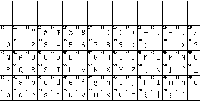
\includegraphics[scale=2.2]{ascii}

\Level 1 {Code pages}

This left the codes with the \index{ascii!8-bit}high bit set
(`\index{ascii!extended}extended \ascii') undefined, and different
manufacturers of computer equipment came up with their own way of
filling them in. These standards were called `\index{code page}code
pages', and IBM gave a standard numbering to them. For instance, code
page~437 is the MS-DOS code page with accented characters for most
European languages, 862~is DOS in Israel, 737~is DOS for Greeks. 

Here is cp473:\\
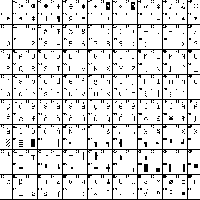
\includegraphics[scale=2.2]{dos437}

MacRoman:\\
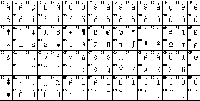
\includegraphics[scale=2.2]{macroman}

and Microsoft cp1252:\\
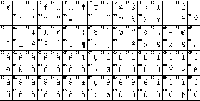
\includegraphics[scale=2.2]{winlatin1}

More code pages are displayed on
\url{http://aspell.net/charsets/codepages.html}.
These diagrams can be generated from Unicode mapping tables, which
look like
\begin{verbatim}
=20     U+0020  SPACE
=21     U+0021  EXCLAMATION MARK
=22     U+0022  QUOTATION MARK
...
=A3     U+00A3  POUND SIGN
=A4     U+20AC  EURO SIGN
=A5     U+00A5  YEN SIGN
...
\end{verbatim}

The international variants were standardized as ISO 646-DE (German),
646-DK (Danish), et cetera. Originally, the dollar sign could still be
replaced by the currency symbol, but after a 1991 revision the dollar
is now the only possibility.

\Level 1 {ISO 8859}

The
different code pages were ultimately standardized as \index{ISO!8859,
Latin alphabets}ISO~8859, with such popular code pages as
8859-\nobreak1 (`Latin~1') for western European,

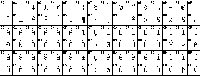
\includegraphics[scale=2.2]{latin1}

8859-\nobreak2 for
eastern, and 8859-\nobreak5 for Cyrillic.

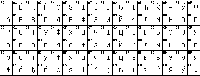
\includegraphics[scale=2.2]{8859-cyrillic}

These ISO standards
explicitly left the first 32 extended positions undefined. Microsoft
code page~1252 uses ISO 8859-\nobreak1.

More useful information about \ascii:
\url{http://jimprice.com/jim-asc.htm}. History of \ascii\ out of
telegraph codes:
\url{http://www.wps.com/projects/codes/index.html}. A~history, paying
attention to multilingual use:
\url{http://tronweb.super-nova.co.jp/characcodehist.html} History as
written by the father of \ascii: Bob Bemer
\url{http://www.bobbemer.com/HISTORY.HTM}.

A good inventory of ISO 8859, Latin-1:
\url{http://www.cs.tut.fi/~jkorpela/latin1/index.html}, with a
discussion by logical grouping:
\url{http://www.cs.tut.fi/~jkorpela/latin1/4.html}.

\Level 1 {DBCS}

Since certain Asian alphabets do not fit in 256 positions, a~system
called the `\index{DBCS}Double Byte Character Set' was invented where
some characters were stored in one, others in two bytes. This is very
messy, since you can not simply write \verb-s++- or \verb+s--+ to
traverse a string. Instead you have to use functions from some library
that understands these encodings. This system is now only of
historical interest.

\Level 0 {Unicode}
\label{sec:unicode}

The systems above functioned quite well as long as you stuck to one
language or writing system. Poor dictionary makers. More or less
simultaneously two efforts started that aimed to incorporate all the
world's character sets in one standard: Unicode standard (originally 2-byte),
and \index{ISO!10646, Unicode}ISO~10646 (oringally 4-byte). Unicode then was
extended, so that it has all numbers up to~\n{10FFFFF}, which is
slightly over a million. 

\Level 1 {ISO 10646 and Unicode}

\index{ISO!10646, Unicode}Two international standards organizations,
the Unicode Consortium and ISO/IEC JTC1/SC2,
started designing a universal standard that was to be a
superset of all existing character sets. These standards are now
synchronized. Unicode has elements
that are not in 10646, but they are compatible where it concerns
straight character encoding.

ISO 10646 defines UCS, the `\index{UCS, Universal Character
  Set}Universal Character Set'. This is in essence a table of official
names
and code numbers for characters. Unicode adds to this rules for hyphenation,
bi-directional writing, and more.

The full Unicode list of code points can be found, broken down by
blocks, online at
\url{http://www.fileformat.info/info/unicode/index.htm}, or
downloadable at \url{http://www.unicode.org/charts/}.

\Level 1 {BMP and earlier standards}

Characters in Unicode are mostly denoted hexadecimally as~\n{U+wxyz},
for instance \n{U+0041} is `Latin Capital Letter~A'.
The range \n{U+0000}--\n{U+007F} (0--127) is identical to US-ASCII
(ISO 646 IRV), and \n{U+0000}--\n{U+00FF} (0--255) is identical to
Latin~1 (ISO 8859-1).

The original 2-byte subset is
now called `\index{BMP}BMP' for Basic Multilingual Plane.

From \url{http://www.hyperdictionary.com/}:
\begin{description}
\item[BMP] (Basic Multilingual Plane) The first plane defined in
  Unicode/ISO 10646, designed to include all scripts in active modern
  use. The BMP currently includes the Latin, Greek, Cyrillic,
  Devangari, hiragana, katakana, and Cherokee scripts, among others,
  and a large body of mathematical, APL-related, and other
  miscellaneous characters. Most of the Han ideographs in current use
  are present in the BMP, but due to the large number of ideographs,
  many were placed in the Supplementary Ideographic Plane.
\item[SIP] (Supplementary Ideographic Plane) The third plane (plane 2)
  defined in Unicode/ISO 10646, designed to hold all the ideographs
  descended from Chinese writing (mainly found in Vietnamese, Korean,
  Japanese and Chinese) that aren't found in the Basic Multilingual
  Plane. The BMP was supposed to hold all ideographs in modern use;
  unfortunately, many Chinese dialects (like Cantonese and Hong Kong
  Chinese) were overlooked; to write these, characters from the SIP
  are necessary. This is one reason even non-academic software must
  support characters outside the BMP.
\end{description}

\Level 1 {Unicode encodings}
\label{sec:uni-encoding}

Unicode is basically a numbered list of characters. When they are used
in a file, their numbers can be encoded in a number of ways. To name
the obvious example: if only the first 128 positions are used, the
long Unicode code point can be truncated to just one byte. Here are a
few encodings:
\begin{description}
\item[UCS-2] Obsolete: this was the original `native' two-byte
  encoding before Unicode was extended.
\item[UTF-32] Little used: this is a four-byte encoding. (UTF stands
  for `UCS Transformation Format'.)
\item[UTF-16] This is the BMP.
\item[UTF-8] A one-byte scheme; details below.
\item[UTF-7] Another one-byte scheme, but now the high bit is always
  off. Certain byte values act as `escape', so that higher values can
  be encoded. Like UTF-1 and SCSU, this encoding is only of historical
  interest.
\end{description}

There is an important practical reason for UTF-8. Encodings such as
UCS-2 are wasteful of space, if only traditional \ascii\ is
needed. Furthermore, they would break software that is expecting to
walk through a file with~\verb-s++- and such. Also, they would
introduce many zero bytes in a file, which would play havoc with Unix
software that uses null-termination for strings. Then there would be
the problem of whether two bytes are stored in low-endian or
high-endian order. For this reason it was suggested to store \n{FE FF}
or \n{FF FE} at the beginning of each file as the `Unicode Byte Order
Mark'. Of course this plays havoc with files such as shell scripts
which expect to find \verb+#!+ at the beginning of the file.

\Level 1 {UTF-8}

UTF-8 is an encoding where the positions up to 127 are encoded `as
such'; higher numbers are encoded in groups of 2 to~6 bytes. (UTF-8 is
standardized as RFC~3629.) In a multi-byte group, the first byte is in
the range 0xC0--0xFD (192--252). The next up to~5 bytes are in the
range 0x80--0xBF (128--191, bit pattern starting with~\n{10}). Note that
$\n{8}=\n{1000}$ and $\n{B}=\n{1011}$, so the highest two bits are
always~\n{10}, leaving six bits for encoding).

\begin{quote}\begin{footnotesize}
\begin{ttfamily}\begin{tabular}{|l|llll|}
\hline
U-00000000 - U-0000007F&\textrm{7 bits}&
0xxxxxxx&&\\
U-00000080 - U-000007FF&$11=5+6$&
110xxxxx&10xxxxxx&\\
U-00000800 - U-0000FFFF&$16=4+2\times6$&
1110xxxx&10xxxxxx&10xxxxxx\\
U-00010000 - U-001FFFFF&$21=3+3\times6$&
11110xxx&\multicolumn{2}{l|}{10xxxxxx (3 times)}\\
U-00200000 - U-03FFFFFF&$26=2+4\times6$&
111110xx&\multicolumn{2}{l|}{10xxxxxx (4 times)}\\
U-04000000 - U-7FFFFFFF&$31=1+5\times6$&
1111110x&\multicolumn{2}{l|}{10xxxxxx (5 times)}\\\hline
  \end{tabular}
\end{ttfamily}
  \end{footnotesize}
\end{quote}

All bites in a multi-byte sequence have their high bit set.

\begin{594exercise}
Show that a UTF-8 parser will not miss more than two characters
if a byte becomes damaged (any number of bits arbitrarily changed).
\end{594exercise}

IETF documents such as
RFC~2277 require support for this encoding in internet
software. Here is a good introduction to UTF-8 use in Unix:
\url{http://www.cl.cam.ac.uk/~mgk25/unicode.html}. The history of
it: \url{http://www.cl.cam.ac.uk/~mgk25/ucs/utf-8-history.txt}.

\Level 1 {Unicode tidbits}

\Level 2 {Line breaking}

See
\url{http://www.cs.tut.fi/~jkorpela/unicode/linebr.html} and
\url{http://www.unicode.org/reports/tr14/}

\Level 2 {Bi-directional writing}

Most scripts are left-to-right, but Arabic and Hebrew run
right-to-left. Characters in a file are stored in `logical order', and
usually it is clear in which direction to render them, even if they
are used mixed. Letters have a `strong' directionality: unless
overridden, they will be displayed in their natural direction. The
first letter of a paragraph with strong direction determines the main
direction of that paragraph.

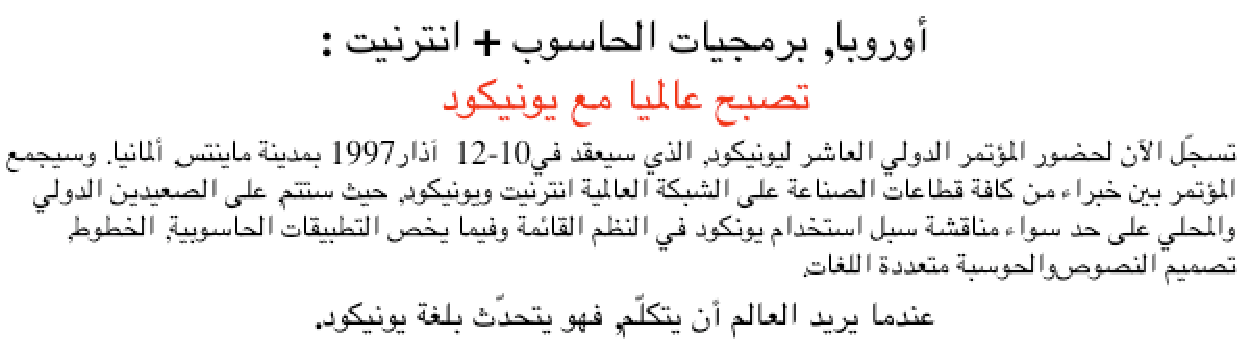
\includegraphics[scale=.6]{arabic-date}

However, when differently directional texts are
embedded, some explicit help is needed. The problem arises with
letters that have only weak directionality. The following is a sketch
of a problematic case.
\begin{quote}
Memory:  he said "I NEED WATER!", and expired.\\
Display: he said "RETAW DEEN I!", and expired.
\end{quote}
If the exclamation mark is to be part of the Arabic quotation, then
the user can select the text `I NEED WATER!' and explicitly mark it as
embedded Arabic (\n{<RLE>} is Right-Left Embedding; \n{<PDF>} Pop
Directional Format), which produces the following result:
\begin{quote}
Memory:  he said "\n{<RLE>}I NEED WATER!\n{<PDF>}", and expired.\\
Display: he said "!RETAW DEEN I", and expired.
\end{quote}
A simpler method of doing this is to place a Right Directional Mark
\n{<RLM>} after the exclamation mark. Since the exclamation mark is now
not on a directional boundary, this produces the correct result.
\begin{quote}
Memory:  he said "I NEED WATER!\n{<RLM>}", and expired.\\
Display: he said "!RETAW DEEN I", and expired.
\end{quote}

For the full definition, see \url{http://www.unicode.org/reports/tr9/}.

\Level 1 {Unicode and oriental languages}
\label{sec:unihan}

`Han unification' is the Unicode strategy of saving space in the
oriental languages (traditional Chinese, simplified Chinese, Japanese,
Korean: `CJK') by recognizing common characters. This idea is not
uncontroversial; see~\url{http://en.wikipedia.org/wiki/Han_unification}.

\Level 0 {More about character sets and encodings}

\Level 1 {Character sets}

Informally, the term `character set' (also `character code' or `code')
used to mean something like `a~table of
bytes, each with a character shape'. With only the English alphabet to
deal with that is a good enough definition. These days, much more general
cases are handled, mapping one octet into several characters, or
several octets into one character. The definition has changed
accordingly:
\begin{quote}
A `\index{charset}\emph{charset} is
a method of   converting a sequence of octets into a sequence of
characters.  This   conversion may also optionally produce additional
control information   such as directionality indicators.
\end{quote}
(From RFC 2978) A~conversion the other way may not exist, since
different octet combinations may map to the same character.  Another
complicating factor is the possibility of switching between character
sets; for instance, \index{ISO 2022}ISO 2022-JP is the standard
\ascii\ character set, but the escape sequence \verb+ESC $ @+ switches
to JIS X 0208-1978.

\Level 1 {From character to encoding in four easy steps}

To disentangle the concepts behind encoding, we need to introduce a
couple of levels:
\begin{description}
\item[ACR] Abstract Character Repertoire: the set of characters to be
  encoded; for example, some alphabet or symbol set. This is an
  unordered set of characters, which can be fixed (the contents of ISO
  8859-1), or open (the contents of Unicode).
\item[CCS] Coded Character Set: a mapping from an abstract character
  repertoire to a set of nonnegative integers. This is what is meant
  by `encoding', `character set definition', or `code page'; the
  integer assigned to a character is its `\index{code point}code
  point'.

  There used to be a drive towards unambiguous abstract character
  names across repertoires and encodings, but Unicode ended this, as
  it provides (or aims to provide) more or less a complete list of
  every character on earth.
\item[CEF] Character Encoding Form: a mapping from a set of
  nonnegative integers that are elements of a CCS to a set of
  sequences of particular code units. A~`\index{code unit}code unit'
  is an integer of a specific binary width, for instance 8 or~16
  bits. A~CEF then maps the code points of a coded character set into
  sequences of code point, and these sequences can be of different
  lengths inside one code page. For instance
\begin{itemize}
\item \ascii\ uses a single 7-bit unit
\item UCS-2 uses a single 16-bit unit
\item DBCS uses two 8-bit units
\item UTF-8 uses one to four 8-bit units.
\item UTF-16 uses a mix of one and two 16-bit code units.
\end{itemize}
\item[CES] Character Encoding Scheme: a reversible transformation from
  a set of sequences of code units (from one or more CEFs to a
  serialized sequence of bytes. In cases such as \ascii\ and UTF-8
  this mapping is trivial. With UCS-2 there is a single `\index{byte
    order mark}byte order mark', after which the code units are
  trivially mapped to bytes. On the other hand, ISO~2022, which uses
  escape sequences to switch between different encodings, is a
  complicated CES.
\end{description}
Additionally, there are the concepts of
\begin{description}
\item[CM] Character Map: a mapping from sequences of members of an
  abstract character repertoire to serialized sequences of bytes
  bridging all four levels in a single operation. These maps are what
  gets assigned MIBenum values by IANA; see section~\ref{sec:mibenum}.
\item[TES] Transfer Encoding Syntax: a reversible transform of encoded
  data. This data may or may not contain textual data. Examples of a
  TES are base64, uuencode, and quoted-printable, which all transform
  a byte stream to avoid certain values.
\end{description}

\Level 1 {A bootstrapping problem}
\label{sec:mibenum}

In order to know how to interpret a file, you need to know what
character set it uses. This problem also occurs in MIME mail encoding
(section~\ref{sec:mime}), which can use many character sets.  Names
and numbers for character sets are standardized by \index{IANA}IANA:
the Internet Assigned Names Authority
(\url{http://www.iana.org/}). However, in what character set do you
write this name down?

Fortunately, everyone agrees on (7-bit) \ascii, so that is what is
used. A~name can be up to 40 characters from us-ascii.

As an example, here is the iana definition of \ascii:
\begin{itemize}
\item[name] \n{ANSI_X3.4-1968}
\item[reference] RFC1345,KXS2
\item[MIBenum] 3
\item[source] ECMA registry
\item[aliases] \n{iso-ir-6}, \n{ANSI_X3.4-1986}, \n{ISO_646.irv:1991},
  \n{ASCII}, \n{ISO646-US}, \n{US-ASCII (preferred MIME name)},
  \n{us}, \n{IBM367}, \n{cp367}, \n{csASCII}
\end{itemize}
The \n{MIBenum} (Management Information Base) is a number assigned by
IANA\footnote{Apparently these numbers derive from the Printer MIB, RFC~1759.}.
The full list of character sets is at
\url{http://www.iana.org/assignments/character-sets},
and RFC 3808 is a memo that describes the IANA Charset MIB.

\Level 1 {Character codes in HTML}

HTML can access unusual characters in several ways:
\begin{itemize}
\item With a decimal numerical code: \verb+&#32;+ is a space
  token. (HTML~4 supports hexadecimal codes.)
\item With a vaguely symbolic name:
  \verb+&copy;+ is the copyright symbol. See
\url{http://www.cs.tut.fi/~jkorpela/HTML3.2/latin1.html} for a list of
symbolic names in Latin-1.
\item The more interesting way is to use an encoding such as UTF-8
  (section~\ref{sec:uni-encoding}) for the file. For this it would be
  nice if the server could state that the file is
\begin{verbatim}
Content-type: text/html;charset=utf-8
\end{verbatim}
  but it is also all right if the file starts with
\begin{verbatim}
<META HTTP-EQUIV="Content-Type" CONTENT="text/html;charset=utf-8">
\end{verbatim}
\end{itemize}

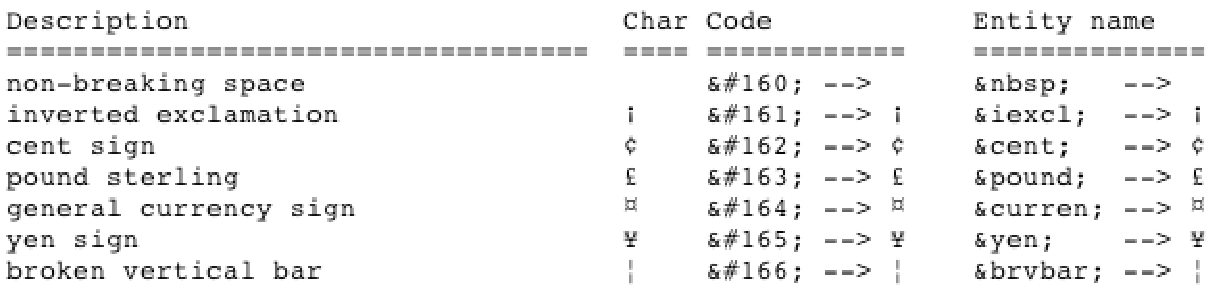
\includegraphics[scale=.6]{latin1-html}

It is requirement that user agents can at least parse the \n{charset}
parameter, which means they have to understand us-ascii.

Open this link in your browser, and additionally view the source:
\url{http://www.unicode.org/unicode/iuc10/x-utf8.html}. How well does
your software deal with it?

See also section~\ref{sec:unicode-font}.

\Level 1 {Characters in email}
\label{sec:mime}

\Level 1 {FTP}

FTP is a very old ARPA protocol. It knows `binary' and `text' mode,
but the text mode is not well defined. Some ftp programs adjust line
ends; others, such as \n{Fetch} on the Mac, actually do code page
translation.

\Level 1 {Character encodings in editors and programming languages}

Software must be rewritten to use character encodings. Windows
NT/2000/XP, including Visual Basic, uses UCS-2 as native string
type. Strings are declared of type \n{wchar_t} instead of \n{char},
and the programmer uses \n{wcslen} instead of \n{strlen}, et
cetera. A~literal string is created as \verb+L"Hello world"+.

\Level 0 {Character issues in \TeX\ / \LaTeX}

\Level 1 {Diacritics}

Original \TeX\ is not very good at dealing with diacritics. They are
implemented as things to put on top of characters, even when, as with
the cedilla, they are under the letter. Furthermore, \TeX\ can not
hypenate a word with accents, since the accent introduces a space in
the word (technically: an explicit kern).
Both problems were remedied to a large extent with the `Cork font
encoding', which contains most accented letters as single
characters. This means that accents are correctly placed by design,
and also that the word can be hyphenated, since the kern has disappeared.

These fonts with accented characters became possible when
\TeX\ version~3 came out around 1990. This introduced full 8-bit
compatibility, both in the input side and in the font addressing.

\Level 1 {\LaTeX\ input file access to fonts}

If an input file for \LaTeX\ is allowed to contain all 8-bit octets,
we get all the problems of compatibility that plagued regular text
files. This is solved by the package \index{inputenc package}\n{inputenc}:
\begin{verbatim}
\usepackage[code]{inputenc}
\end{verbatim}
where \n{codes} is \n{applemac}, \n{ansinew}, or various other
\index{code page}code pages.

This package makes all unprintable \ascii\ characters, plus the codes
over~127, into active characters. The definitions are then dynamically
set depending on the code page that is loaded.

\Level 1 {\LaTeX\ output encoding}

The \n{inputenc} package does not solve the whole problem of producing
a certain font character from certain keyboard input. It only mapped a
byte value to the \TeX\ command for producing a character. To map such
commands to actual code point in a font file, the \TeX\ and
\LaTeX\ formats contain lines such as
\begin{verbatim}
\chardef\i="10
\end{verbatim}
declaring that the dotless-i is at position~16. However, this position
is a convention, and other people --~type manufacturers~-- may put it
somewhere else.

This is handled by the \index{font encoding}`font encoding'
mechanism.
The various people working on the \LaTeX\ font schemes have devised a
number of standard font encodings. For instance, the
\index{OT1}\n{OT1} encoding corresponds to the original 128-character
set. The \index{T1}\n{T1} encoding is a 256-character extension
thereof, which includes most accented characters for Latin alphabet
languages.

A font encoding is selected with
\begin{verbatim}
\usepackage[T1]{fontenc}
\end{verbatim}
A font encoding definition contains lines such as
\begin{verbatim}
\DeclareTextSymbol{\AE}{OT1}{29}
\DeclareTextSymbol{\OE}{OT1}{30}
\DeclareTextSymbol{\O}{OT1}{31}
\DeclareTextSymbol{\ae}{OT1}{26}
\DeclareTextSymbol{\i}{OT1}{16}
\end{verbatim}

\Level 1 {Virtual fonts}

\begin{594exercise}
What does an \n{ALT} key do?
\end{594exercise}

\begin{594exercise}
What is \ebcdic? What is the basic idea?
\end{594exercise}

\begin{594exercise}
Find the Unicode definition. Can you find an example of a
character that has two functions, but is not defined as two
characters? Find two characters that are defined seperately for
compatibility, but that are defined equivalent.
\end{594exercise}

\begin{594exercise}
ISO 8859 has the `non-breaking space' at position~\n{A0}. How
does \TeX\ handle the nbsp? How do \TeX, HTML, Latin-1, MS Word, et
cetera handle multiple spaces? Discuss the pros and cons.  
\end{594exercise}
